\documentclass[11pt]{article}

\usepackage{amsmath}
\usepackage{amssymb}
\usepackage{graphicx}
\usepackage{hyperref}

\title{LSC Framework v1.2.0: Computational Extension and Reproducibility Update}
\author{LuciferSun \\ Independent Research}
\date{2026}

\begin{document}

\maketitle

\begin{abstract}
This release documents version 1.2.0 of the LSC framework, an incremental update focused on reproducibility, computational modeling, and formal preprint preparation. The model is presented as a phenomenological framework for studying gravitationally coupled corrections to neutrino oscillation observables. We include the effective LSC Hamiltonian structure, a reproducible numerical evaluation of the LSC potential as a function of radius, diagnostic resonance-condition plots, and source code for regenerating the figures. The work is not presented as confirmed new physics; it is a testable computational ansatz intended for independent review and falsification.
\end{abstract}

\section{Introduction}

The LSC research line explores whether phenomenological corrections to neutrino propagation and detector-level observables can be organized in a mathematically explicit and computationally reproducible way. Earlier public materials documented the conceptual structure of the framework and its relation to neutrino anomalies, gravitational effects, and detector-response modeling.

Version 1.2.0 is an incremental release. Its primary purpose is to make the computational layer explicit: the release includes Python scripts, generated figures, a reproducibility package, and metadata suitable for Zenodo archival. The public project website is available at
\begin{center}
\url{https://luciferprosun.github.io/akasha-chronicles}.
\end{center}

\section{Theory}

The effective flavor-evolution structure is written as
\begin{equation}
 H_{\rm eff}=H_{\rm vac}+H_{\rm matter}+H_{\rm grav}+H_{\rm LSC}.
\end{equation}
The standard vacuum term is
\begin{equation}
 H_{\rm vac}=\frac{1}{2E}U M^2 U^\dagger,
\end{equation}
where $U$ is the PMNS matrix, $M^2$ is the neutrino mass-squared matrix, and $E$ is the local neutrino energy used in the effective description. The matter term is represented in the usual diagonal approximation,
\begin{equation}
 H_{\rm matter}=\operatorname{diag}(V_e,0,0),
 \qquad
 V_e=\sqrt{2}G_F n_e .
\end{equation}

The LSC correction is modeled phenomenologically as
\begin{equation}
 H_{\rm LSC}=\alpha_{\rm LSC}
 \left(\frac{GM}{r c^2}\right)
 \left(\frac{E}{1~{\rm PeV}}\right),
\end{equation}
where $\alpha_{\rm LSC}$ is the dimensionless LSC coupling, $G$ is Newton's constant, $M$ is the source mass, $r$ is the radial coordinate, and $c$ is the speed of light. In this release, $H_{\rm LSC}$ is used as an effective potential-like contribution rather than as a microscopic derivation.

The resonance diagnostic is written in the MSW-like form
\begin{equation}
 \Delta m^2\cos(2\theta)=2E\left(V_{\rm matter}+V_{\rm LSC}\right).
\end{equation}
The standard limit is recovered when $\alpha_{\rm LSC}\rightarrow 0$.

\section{Computational Extension}

The computational component evaluates the effective LSC potential over a radial grid near a compact gravitational source. The numerical model computes
\begin{equation}
 V_{\rm LSC}(r,E)=\alpha_{\rm LSC}
 \left(\frac{GM}{r c^2}\right)
 \left(\frac{E}{1~{\rm PeV}}\right)E_{\rm scale},
\end{equation}
where $E_{\rm scale}=1~{\rm eV}$ is an explicit normalization used to express the dimensionless ansatz as an effective potential for plotting.

The resonance diagnostic is
\begin{equation}
 R(r)=2E\left[V_{\rm matter}+V_{\rm LSC}(r,E)\right],
\end{equation}
with reference scale
\begin{equation}
 R_0=\Delta m^2\cos(2\theta).
\end{equation}

The release contains two reproducibility scripts:
\begin{itemize}
 \item \texttt{code/simulation.py}: computes the numerical arrays and writes JSON output.
 \item \texttt{code/plot\_results.py}: regenerates the release figures.
\end{itemize}

\section{Results}

Figure~\ref{fig:lsc-potential} shows the numerical LSC potential as a function of radius. The reference behavior follows the compactness factor $GM/(rc^2)$ and decreases monotonically with distance.

\begin{figure}[ht]
\centering
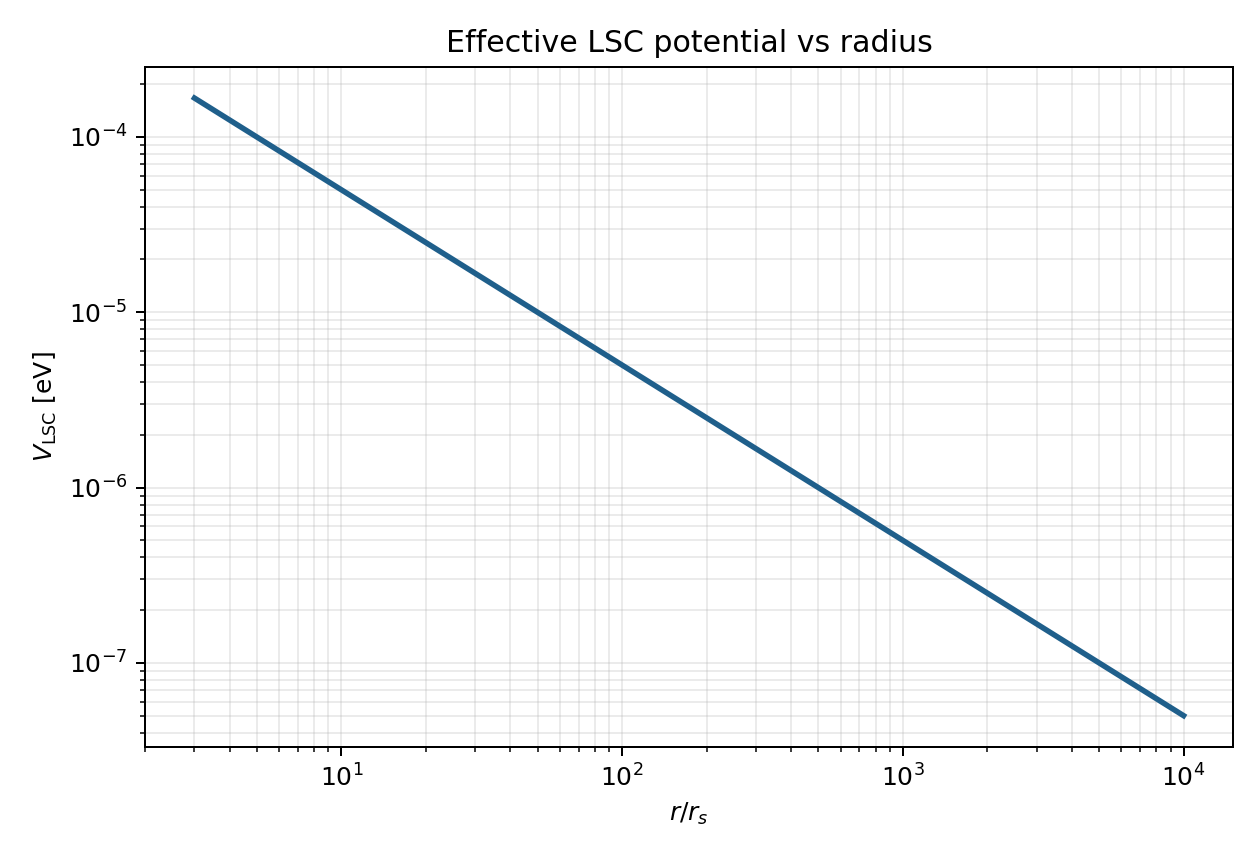
\includegraphics[width=0.82\linewidth]{../figures/lsc_potential.png}
\caption{Effective LSC potential as a function of radius for the reference numerical parameter set.}
\label{fig:lsc-potential}
\end{figure}

Figure~\ref{fig:resonance} shows the resonance-condition diagnostic. The plotted comparison is not a claim of experimental confirmation. It indicates where the selected phenomenological parameters would become numerically relevant inside the simplified computational model.

\begin{figure}[ht]
\centering
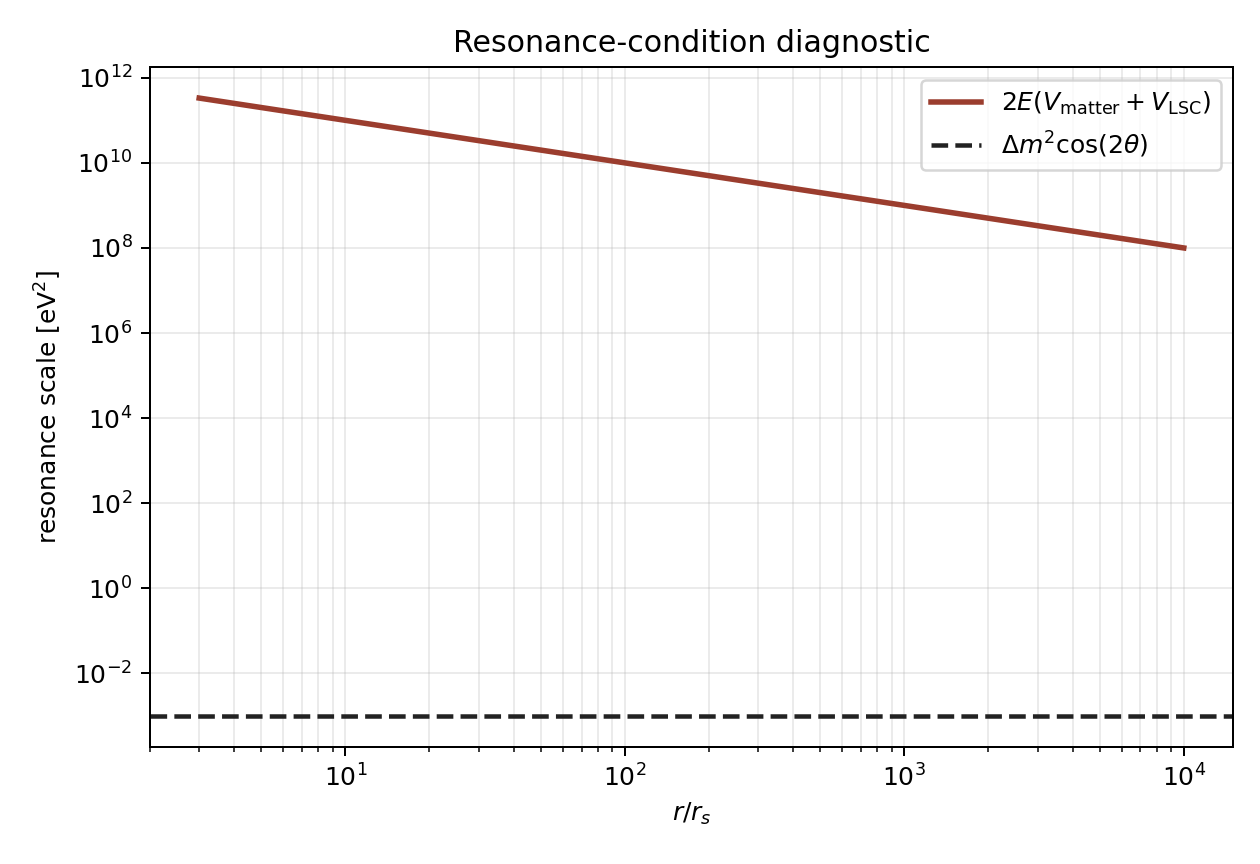
\includegraphics[width=0.82\linewidth]{../figures/resonance_plot.png}
\caption{Resonance-condition diagnostic comparing $2E(V_{\rm matter}+V_{\rm LSC})$ with $\Delta m^2\cos(2\theta)$.}
\label{fig:resonance}
\end{figure}

\section{Discussion}

This release improves the reproducibility status of the LSC framework by separating the computational demonstration from broader theoretical interpretation. The model remains phenomenological and requires independent review, parameter constraints, and comparison with established neutrino data sets. The numerical examples are intended as diagnostics and should not be read as a global fit.

The release is suitable for archival because it includes source code, figures, metadata, and a compiled paper. It is also suitable as supporting material for a formal preprint submission.

\section{Submission Status}

The work has been submitted to arXiv. It is currently awaiting endorsement for category access. A preprint and reproducibility package are publicly available via Zenodo, with this release intended to document the current model state, computational extension, and reproducibility materials.

The endorsement request link associated with the current arXiv account process is:
\begin{center}
\url{https://arxiv.org/auth/endorse?x=7KLAMS}.
\end{center}

\section{Conclusion}

LSC Framework v1.2.0 provides an incremental, reproducible update to the LSC model line. It adds numerical modeling, generated figures, release metadata, and a clear arXiv submission-status record while maintaining a conservative scientific interpretation.

\begin{thebibliography}{9}
\bibitem{wolfenstein1978}
L. Wolfenstein, ``Neutrino oscillations in matter,'' Phys. Rev. D 17, 2369 (1978).

\bibitem{msw1985}
S. P. Mikheyev and A. Yu. Smirnov, ``Resonant amplification of neutrino oscillations in matter and solar neutrino spectroscopy,'' Sov. J. Nucl. Phys. 42, 913 (1985).

\bibitem{cardall1997}
C. Y. Cardall and G. M. Fuller, ``Neutrino oscillations in curved spacetime: An heuristic treatment,'' Phys. Rev. D 55, 7960 (1997).

\bibitem{fornengo1997}
N. Fornengo, C. Giunti, C. W. Kim, and J. Song, ``Gravitational effects on the neutrino oscillation,'' Phys. Rev. D 56, 1895 (1997).

\bibitem{best2022}
V. V. Barinov et al., ``Results from the Baksan Experiment on Sterile Transitions (BEST),'' Phys. Rev. Lett. 128, 232501 (2022).

\bibitem{zenodo60}
LuciferSun, ``LSC 6.0 public record,'' Zenodo, \url{https://zenodo.org/records/19780616}.

\bibitem{github60}
LuciferSun, ``LSC 6.0 GitHub release,'' \url{https://github.com/luciferprosun/LSC-6.0/releases/tag/v1.0.0}.
\end{thebibliography}

\end{document}
